%% SANER 2027 -- Reproducibility Studies and Negative Results (RENE) Track
%% Limit: 10 pages including figures and appendices, plus up to 2 pages
%%        containing ONLY references.
%% Formatting per SANER guidance: IEEEtran, 10pt, conference option, and
%%        WITHOUT the compsoc or compsocconf option.
%% Double-anonymous: no author names, affiliations, acknowledgments, or
%%        identifying links anywhere in this file.
\documentclass[10pt,conference]{IEEEtran}
\IEEEoverridecommandlockouts

\usepackage{cite}
\usepackage{amsmath,amssymb}
\usepackage{booktabs}
\usepackage{graphicx}
\usepackage{xcolor}
\usepackage{tikz}
\usetikzlibrary{arrows.meta,positioning,patterns}
\usepackage[hidelinks]{hyperref}

\newcommand{\killk}[1]{Kill@#1}
\definecolor{oaccent}{HTML}{2F5D8C}
\definecolor{ofail}{HTML}{A5372F}
\definecolor{opass}{HTML}{2C6B4D}
\definecolor{orule}{HTML}{B9C2CE}

\begin{document}

\title{A Development Gain That Did Not Survive Locking:\\
Negative and Inconclusive Results from an\\
LLM-Based Mutation Test Generation Pipeline}

\author{\IEEEauthorblockN{}\IEEEauthorblockA{}}

\maketitle

\begin{abstract}
Supervised fine-tuning (SFT) of a small code LLM for mutation test generation
produced a large apparent gain on the panel used to select its checkpoints, and
a much smaller gain that did not meet a significance threshold fixed in advance
on a locked validation split. On the selection panel, \killk{8} rose from
$0.605166$ to $0.695572$. On the locked split the paired difference was
$+3.4346$ percentage points (450/757 to 476/757) with an exact two-sided
McNemar $p = 0.0783$, against a predeclared requirement of $p < 0.01$. Under
the rule frozen before either arm ran, the untrained base model was retained.
Over the same locked comparison, the fraction of reference-valid candidates
fell by $11.8726$ points while parse and execution validity did not degrade:
the tuned model wrote more mutant-killing tests that more often failed against
the correct implementation. We report these results as negative and
inconclusive evidence respectively, and we are explicit that a non-significant
difference is not evidence of no difference. We also report an evaluation-
integrity failure. A one-time final measurement was authorized and consumed
without producing any measurement, because a record-admission rule in the
final-run path rejected records that the established evaluator had always
excluded later by scope. The defect was reproducible on permitted splits and
had never been executed against real data. The resulting safeguard --- a
receipt-bound, full-scale rehearsal on a permitted split --- reproduced a
previously measured value exactly, demonstrating pipeline execution fidelity
without touching the consumed split. We distil the episode into actionable
controls for anyone measuring LLM-based testing tools.
\end{abstract}

\begin{IEEEkeywords}
negative results, reproducibility, mutation testing, large language models,
test generation, evaluation integrity, data leakage
\end{IEEEkeywords}

\section{Introduction}

A measurement pipeline for LLM-based test generation has two ways to mislead.
It can report a real number about the wrong population, and it can report a
number that its own code never actually computed the way the paper says. This
paper reports one instance of each, from a single project, with every figure
traceable to an artifact frozen before the corresponding measurement ran.

The substantive result is negative in the specific sense the RENE track asks
for. Supervised fine-tuning of a 1.5B-parameter code model for mutation test
generation produced a $+9.04$ point \killk{8} gain on the panel that had been
used to select its checkpoints, and $+3.4346$ points on a locked split that had
not been used to select a checkpoint, tune a prompt, or set a threshold. The
locked difference did not meet a significance threshold
fixed in advance, so the predeclared rule retained the untrained base model.
The same comparison shows a substantial regression in candidate
\emph{reference validity} --- whether a generated test passes against the
correct implementation --- with no accompanying regression in parsing or
execution. A tuned model that kills more mutants while more often failing the
reference is not obviously a better test generator, and a pipeline that reports
only \killk{k} would not have seen it.

The methodological result is an evaluation-integrity failure and its repair. A
one-time final measurement, protected by a single-use authorization and a
hash-bound receipt, was spent without producing any measurement. The immediate
cause was a record-admission rule in the final-run path that required every
record in a split to carry a non-empty set of fields, applied \emph{before} the
scope filter that the established evaluator had always applied first. Records
legitimately carrying blank fields were therefore rejected rather than excluded.
The defect reproduced on permitted splits at any time and cost nothing to find
there; it survived because the component was deliberately unreachable until the
authorization was spent, and so had never been executed against real data.

\subsection*{Contributions}

\begin{enumerate}
  \item A quantified instance of development-to-locked shrinkage in LLM-based
        mutation test generation: a $+9.04$ point selection-panel gain
        corresponding to $+3.4346$ points on a locked split, with the locked
        result failing a predeclared significance criterion
        (Section~\ref{sec:rq1}).
  \item Evidence that \killk{k} and candidate reference validity moved in
        opposite directions under SFT, isolated from parse and execution
        validity (Section~\ref{sec:rq2}).
  \item An analysis of how parsing semantics, retained raw outputs and split
        isolation determine whether a reported number can be interpreted at all
        (Section~\ref{sec:rq3}).
  \item A post-mortem of a consumed one-time measurement, and a
        receipt-bound full-scale rehearsal that reproduced a prior value exactly
        on a permitted split (Section~\ref{sec:rq4}).
  \item A set of controls that would have caught each failure, stated as
        checks rather than principles (Section~\ref{sec:lessons}).
\end{enumerate}

\section{Study Design}
\label{sec:design}

\subsection{System under measurement}

The measured system generates unit tests intended to distinguish a mutated
function from its correct implementation. The generator is
\texttt{Qwen2.5-Coder-1.5B-Instruct}, pinned at an immutable revision. All
measurements reported here run under one named generation protocol, frozen and
identified by digest: eight candidates per target, temperature $0.7$, top-$p$
$0.9$, seed 42, whole-output candidate parsing, raw-output retention, a 1024
token completion limit, a 3072 token sequence limit, no reranking and no
feedback rounds. Four arms were evaluated under one contract digest and one
evaluation-scope digest, recorded as identical across all four.

The primary metric is \killk{k}: the fraction of target functions for which at
least one of the first $k$ generated candidates, in raw generation order, kills
the mutant. We also report \emph{parse validity} (the candidate is extractable
and syntactically usable), \emph{execution validity} (it runs without
infrastructure error), and \emph{reference validity} (it passes against the
correct implementation). Reference validity is the quality signal most easily
lost when only \killk{k} is reported, because a test that fails everything kills
every mutant.

\subsection{Splits and their roles}

Figure~\ref{fig:splits} shows the four splits and, more importantly, what each
one is permitted to support. The distinction that matters for this paper is
between the panel that \emph{selected} checkpoints and the split that was not
used to select a checkpoint, tune a prompt, or set a threshold, and that
determined the predeclared promotion decision.

\begin{figure}[t]
\centering
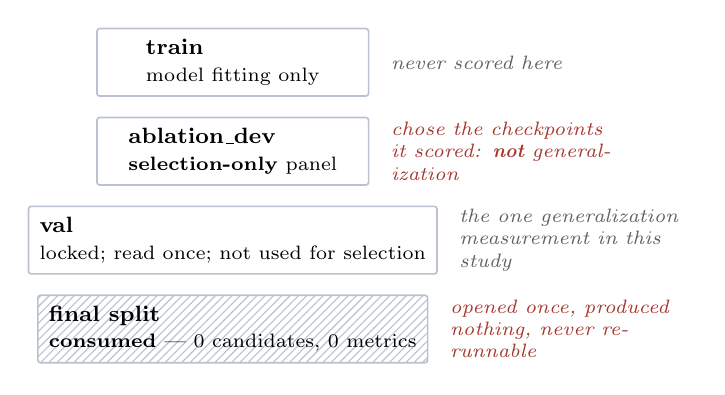
\begin{tikzpicture}[
  font=\footnotesize,
  box/.style={draw=orule,line width=0.6pt,rounded corners=1pt,
              minimum width=3.45cm,minimum height=0.82cm,align=left,
              inner sep=4pt},
  lbl/.style={font=\scriptsize\itshape,text=black!62}
]
\node[box] (train) {\textbf{train} \\ \scriptsize model fitting only};
\node[box,below=2.5mm of train] (dev)
  {\textbf{ablation\_dev} \\ \scriptsize \textbf{selection-only} panel};
\node[box,below=2.5mm of dev] (val)
  {\textbf{val} \\ \scriptsize locked; read once; not used for selection};
\node[box,below=2.5mm of val,pattern=north east lines,
      pattern color=orule] (test)
  {\textbf{final split} \\ \scriptsize \textbf{consumed} --- 0 candidates,
   0 metrics};

\node[lbl,right=1.5mm of train.east,text width=2.9cm]
  {never scored here};
\node[lbl,right=1.5mm of dev.east,text width=2.9cm,text=ofail]
  {chose the checkpoints it scored: \textbf{not} generalization};
\node[lbl,right=1.5mm of val.east,text width=2.9cm]
  {the one generalization measurement in this study};
\node[lbl,right=1.5mm of test.east,text width=2.9cm,text=ofail]
  {opened once, produced nothing, never re-runnable};
\end{tikzpicture}
\caption{Split roles. For the consumed final split we give neither its size, its
membership, its record counts nor any performance score. The two zeros shown are
a historical fact about the authorized attempt --- it generated zero candidates
and zero reportable metrics --- not a measurement of the split. No result in this
paper derives from it.}
\label{fig:splits}
\end{figure}

\subsection{Predeclared decision rule}

Before either locked arm ran, a promotion rule was committed to a hash-bound
receipt. Its first criterion required all three of: a \killk{8} gain of at least
$+3.0$ points, a net gain of at least $15$ functions, and an exact two-sided
McNemar $p < 0.01$. Further criteria bounded the permitted regression in
reference validity, parse and execution validity, and candidate diversity. The
rule was fixed in advance precisely so that a borderline $p$ could not be
renegotiated afterwards, which is what a threshold is for.

\section{RQ1: How much did the selection panel overstate?}
\label{sec:rq1}

Table~\ref{tab:main} gives the result. On the selection panel the best arm
reached $\killk{8} = 0.695572$ against a base of $0.605166$, a gain of $9.04$
points. On the locked split the same checkpoint reached $0.628798$ against a
base of $0.594452$: $+3.4346$ points, a factor of roughly $2.6$ smaller.

\begin{table}[t]
\caption{Main results. The two blocks are \textbf{not} comparable quantities:
the development block selected the checkpoints it scores.}
\label{tab:main}
\centering
\footnotesize
\begin{tabular}{@{}llrrr@{}}
\toprule
Panel & Arm & \killk{8} & Fns & Wilson 95\% \\
\midrule
\multicolumn{5}{@{}l}{\textit{Development --- selection-only, $n=542$}}\\
& base   & 0.605166 & 328 & [0.5634, 0.6454] \\
& A@150  & 0.690037 & 374 & [0.6499, 0.7275] \\
& A@431  & 0.695572 & 377 & [0.6556, 0.7328] \\
& B@150  & 0.658672 & 357 & [0.6178, 0.6973] \\
\midrule
\multicolumn{5}{@{}l}{\textit{Locked validation --- not used for selection, $n=757$}}\\
& base   & 0.594452 & 450 & [0.5591, 0.6289] \\
& A@431  & 0.628798 & 476 & [0.5938, 0.6625] \\
\midrule
\multicolumn{5}{@{}l}{\textit{Paired locked difference, A@431 vs.\ base}}\\
& gained/lost/net   & \multicolumn{3}{r}{$+114$ / $-88$ / $+26$} \\
& \killk{8} delta   & \multicolumn{3}{r}{$+3.4346$ points} \\
& McNemar exact $p$ & \multicolumn{3}{r}{$0.0783$} \\
& predeclared requirement & \multicolumn{3}{r}{$p < 0.01$ --- \textbf{not met}} \\
& decision          & \multicolumn{3}{r}{\textbf{retain base model}} \\
\bottomrule
\end{tabular}
\end{table}

Two readings must be kept apart. The shrinkage is real and it is exactly what
selection bias predicts: the development panel chose the checkpoint it then
scored, so its figure is a selection statistic. The locked figure is the only
generalization measurement in this study, and it is \emph{positive}.

What the locked figure does not do is establish an improvement at the evidential
standard set in advance. $p = 0.0783$ against a required $p < 0.01$ means the
data are insufficient to conclude an effect at that standard. It does
\textbf{not} mean the effect is absent, and we do not claim that
\cite{wasserstein2016asa,amrhein2019retire}. The honest summary is that the
question is undetermined at this sample size, and it cannot now be resolved on
this split: once a split has been used to make a decision, re-measuring it to
obtain a different decision is no longer a held-out measurement.

Two further cautions follow from the design. First, $n = 757$ paired targets
with 362 killed by both arms and 193 by neither leaves 202 discordant pairs,
which is the effective sample for McNemar's test \cite{mcnemar1947note}; with
114 versus 88 the test is simply not decisive. Second, a single paired
observation of shrinkage on one task, one model and one corpus does not
establish a general ratio, and we do not offer $2.6\times$ as one.

\section{RQ2: \killk{k} against candidate validity}
\label{sec:rq2}

Table~\ref{tab:validity} shows a trade-off that a \killk{k}-only report would
have hidden. Across the locked comparison, reference validity fell from
$0.452114$ to $0.333388$, a change of $-11.8726$ points, and the number of
target functions with \emph{any} reference-valid candidate fell from 675 to 566.
Over the same comparison, parse validity rose slightly and execution validity
rose by $1.3870$ points.

\begin{table}[t]
\caption{Candidate validity. Parse and execution did not regress, which makes
the reference-validity drop specific rather than general degradation.}
\label{tab:validity}
\centering
\footnotesize
\begin{tabular}{@{}llrrr@{}}
\toprule
Panel & Arm & Parse & Exec. & \textbf{Reference} \\
\midrule
\multicolumn{5}{@{}l}{\textit{Development --- selection-only}}\\
& base   & 0.983395 & 0.948570 & \textbf{0.565498} \\
& A@150  & 0.997463 & 0.975092 & \textbf{0.458487} \\
& A@431  & 0.998155 & 0.993081 & \textbf{0.455028} \\
& B@150  & 0.998155 & 0.973478 & \textbf{0.448801} \\
\midrule
\multicolumn{5}{@{}l}{\textit{Locked validation}}\\
& base   & 0.987285 & 0.928336 & \textbf{0.452114} \\
& A@431  & 0.988771 & 0.942206 & \textbf{0.333388} \\
& delta  & $+0.1486$ & $+1.3870$ & $\mathbf{-11.8726}$ \\
\bottomrule
\end{tabular}
\end{table}

The direction is consistent across all four development arms, so it is a
property of this supervision family rather than of one checkpoint. The
mechanism we can evidence is structural rather than semantic: a test that fails
against every implementation kills every mutant it is scored against, so
\killk{k} rewards aggressiveness that reference validity penalises. Because
parse and execution validity did not fall, the regression is not explained by
the tuned model emitting more malformed or non-running code.

We are careful about the strength of this claim. We observed the trade-off; we
did not manipulate it. Whether a different supervision recipe, a
validity-aware objective or a reference-validity gate at generation time would
remove it is unmeasured here.

\section{RQ3: What makes a reported number interpretable}
\label{sec:rq3}

Three pipeline properties determined whether the numbers above could be read at
all, and each was, at some point, wrong in a way that produced plausible output.

\paragraph{Parsing semantics decide what was measured}
The generator's candidate extraction has two modes: taking the first assertion
found, or taking the whole output. These score different artifacts. An earlier
version of the final-run path never set the mode explicitly and inherited the
legacy default, which would have produced a plausible number under one parser
while the receipt claimed another. Parsing mode is not an implementation
detail; it is part of the measurement's definition, and it belongs in the
frozen record alongside the seed.

\paragraph{Retained raw outputs are what makes a result auditable}
Every candidate slot retains its raw model output and a digest of it. This is
what allowed an independent recomputation of all $4{,}336$ output digests in the
rehearsal, and what allows a disputed score to be re-examined without
regenerating anything. A pipeline that stores only verdicts cannot distinguish a
scoring bug from a model behaviour.

\paragraph{Split isolation must be enforced by construction}
Development, locked and final splits are only meaningfully different if the code
cannot reach the wrong one. In our case the loader that guarded the final split
gated on \emph{authorization} --- a fact that, once recorded, never expires ---
rather than on whether anything remained to measure. This is a category error
that any project using one-time measurements can make: a permission check is
not an exhaustion check.

We also note a leakage concern specific to this task family. Where targets are
drawn from public benchmarks, a model may reproduce a known assertion rather
than derive one \cite{yang2023rephrased,kapoor2023leakage}. The project
separated assertion \emph{form} from assertion \emph{value} in classification
for exactly this reason, so that a gain could not be silently credited to the
wrong mechanism.

\section{RQ4: A rehearsal that reproduces without re-measuring}
\label{sec:rq4}

\subsection{What was lost}

A one-time final measurement was authorized and attempted. It reached
\texttt{failed\_after\_authorization}: the single-use authorization was spent
and the run raised while admitting records, before generating anything. It
produced \textbf{zero candidates and zero reportable metrics}. No prompt was
rendered from a record of that split, nothing was generated, nothing was scored.
The split is consumed and may never be rerun, because a split that has been
opened is no longer held out regardless of what it produced.

The cause was narrow and entirely reproducible elsewhere. The final-run loader
required a fixed set of record fields to be non-empty on \emph{every} record in
a split and raised before returning any of them. Records of one execution mode
in this corpus legitimately carry some of those fields blank; the established
evaluator had always loaded the whole split and \emph{then} scoped scoring to
the relevant mode. The final path inverted that order, so it refused exactly the
records the pipeline was always going to exclude. Running the same selector
against permitted splits reproduces the rejection immediately.

Critically, a repository-only exemption would still have been wrong: on the
locked split three records of the \emph{scored} mode also carry one of those
fields blank, and they were measured. The requirement had to become
mode-dependent, not merely tolerant of one record class.

\subsection{Why the audits did not find it}

The component had been reviewed repeatedly. Six generations of the readiness
receipt were each superseded after an audit found a genuine defect, and a large
test suite passed throughout. Every one of those defects was in something
\emph{recorded} but never \emph{executed}. The pre-authorization smoke test
proved the \emph{generator} on two synthetic records; it did not prove the
\emph{loader} on a real split. The component was deliberately unreachable until
the authorization was spent --- and that design is precisely what kept it
untested.

\begin{figure}[t]
\centering
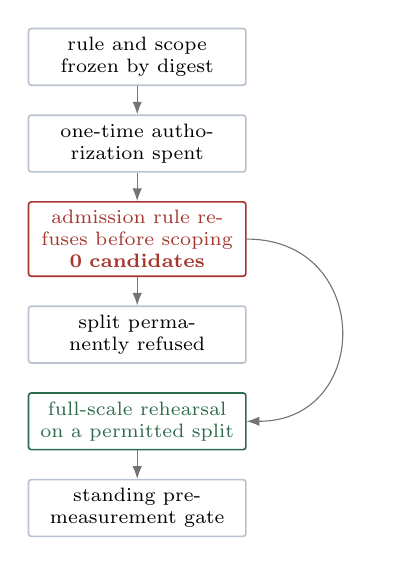
\begin{tikzpicture}[
  font=\scriptsize,
  n/.style={draw=orule,line width=0.6pt,rounded corners=1pt,
            text width=2.55cm,align=center,inner sep=3pt,minimum height=0.72cm},
  a/.style={-{Latex[length=1.6mm]},draw=black!55}
]
\node[n] (freeze) {rule and scope frozen by digest};
\node[n,below=3.6mm of freeze] (auth) {one-time authorization spent};
\node[n,below=3.6mm of auth,draw=ofail,text=ofail]
  (fail) {admission rule refuses before scoping\\\textbf{0 candidates}};
\node[n,below=3.6mm of fail] (refuse) {split permanently refused};
\node[n,below=3.6mm of refuse,draw=opass,text=opass]
  (reh) {full-scale rehearsal on a permitted split};
\node[n,below=3.6mm of reh] (gate) {standing pre-measurement gate};
\draw[a] (freeze) -- (auth);
\draw[a] (auth) -- (fail);
\draw[a] (fail) -- (refuse);
\draw[a] (fail.east) .. controls +(1.6,0) and +(1.6,0) .. (reh.east);
\draw[a] (reh) -- (gate);
\end{tikzpicture}
\caption{From the consumed measurement to the safeguard. No record, identifier
or payload from the consumed split appears in this paper.}
\label{fig:incident}
\end{figure}

\subsection{The rehearsal}

The repair was not only to fix the admission rule but to remove the condition
that made it untestable. We built a mode-aware admission function that
partitions by execution mode first and applies field requirements only to the
records that will actually be scored, importing the mode semantics from the
established evaluator rather than restating them. We then ran the entire
measurement path --- receipt verification, admission, scoping, generation,
whole-output parsing, safe execution, raw-output retention, progress writing and
scoring --- at full scale on a permitted split, under a hash-bound receipt.

The rehearsal scoped 594 requested records to 542 scored targets with 52
excluded by mode and zero admission errors, generated $4{,}336$ candidates in
271 batches of two, retained $4{,}336$ raw outputs with $4{,}336$ digests, and
reported zero missing and zero mismatched; an independent recomputation of every
digest also found zero mismatches. It completed in $577.753$ seconds with exit
status 0, wrote no weights, loaded no adapter and performed no training. Its
\killk{8} was $0.605166$ --- identical to the previously recorded value for the
same model on the same split, under the same evaluation-scope digest.

That exact reproduction is the point, and its scope must be stated precisely.
It is evidence that the rebuilt path computes the same number as the path that
produced the historical value: \emph{execution fidelity}. It is not a
model-performance result, not a generalization estimate, not a selection
result, and not a substitute for the measurement that was lost. The rehearsal
receipt records \texttt{final\_test\_measurement: false},
\texttt{eligible\_for\_model\_selection: false} and
\texttt{supports\_performance\_claim: false} as machine-checkable fields, and
the runner refuses any receipt that does not carry them.

\section{What Can and Cannot Be Claimed}
\label{sec:claims}

Table~\ref{tab:claims} separates the three categories that this track exists to
keep apart.

\begin{table}[t]
\caption{Claim status. The unavailable block is not a list of future work; it
is a list of things this study cannot support.}
\label{tab:claims}
\centering
\footnotesize
\begin{tabular}{@{}p{0.94\columnwidth}@{}}
\toprule
\textbf{Established} \\
\midrule
Selection-panel \killk{8} rose $0.605166 \to 0.695572$; the same checkpoint gave
$0.594452 \to 0.628798$ on the locked split. \\
The paired locked difference was $+3.4346$ points, $+114/-88$, net $+26$,
McNemar exact $p = 0.0783$. \\
The predeclared criterion required $p < 0.01$; it was not met, and the base
model was retained. \\
Reference validity fell $11.8726$ points on the locked comparison while parse
and execution validity did not regress. \\
A full-scale permitted-split rehearsal reproduced a prior \killk{8} of
$0.605166$ exactly, with complete raw-output integrity and no weights written. \\
The one-time final measurement was consumed, producing zero candidates and zero
metrics. \\
\midrule
\textbf{Inconclusive} \\
\midrule
Whether SFT improves \killk{8} on unseen data: undetermined at this sample size.
The point estimate is positive; the predeclared threshold was not met. This is
not evidence of no effect. \\
Whether the reference-validity regression is intrinsic to this objective or an
artifact of one recipe. \\
Whether the observed shrinkage ratio generalises beyond this task, model and
corpus. \\
\midrule
\textbf{Unavailable} \\
\midrule
No final-test result exists for any arm. \\
No native repository-level kill rate exists; records of that mode are excluded
from every rate reported here. \\
No comparison against any external baseline tool exists; none was bundled or
executed in any measurement reported here. \\
Both held-out panels are expended: one on selection, one by the consumed
attempt. \\
\bottomrule
\end{tabular}
\end{table}

\section{Actionable Lessons}
\label{sec:lessons}

These are stated as checks because principles are easy to agree with and hard to
fail.

\begin{enumerate}
  \item \textbf{Freeze the decision rule, with its threshold, in a hashed
        artifact before any arm runs.} Our locked $p = 0.0783$ sat close enough
        to a boundary that a rule written afterwards would have been suspect
        whichever way it fell.
  \item \textbf{Report at least one validity metric alongside \killk{k}.} The
        regression we found is invisible to a kill-rate-only report and moves in
        the opposite direction to the headline.
  \item \textbf{Bind sources by per-file digest, not a whole-tree hash.} A
        tree hash changes for reasons unrelated to the measurement and trains
        people to ignore it.
  \item \textbf{Record both a raw and a line-ending-normalised source digest.}
        Otherwise an identical checkout on another platform appears to be
        different code.
  \item \textbf{Make the scope filter run before the admission check, and
        derive both from one definition.} Two statements of the same rule drift;
        ours drifted into an unrecoverable failure.
  \item \textbf{Fail the whole split, not the offending record.} A silently
        dropped target changes the denominator of every rate.
  \item \textbf{Execute the full path on permitted data at full scale before any
        irreversible measurement.} A smoke test on synthetic records proves the
        generator, not the pipeline. This is the single control that would have
        prevented our loss outright.
  \item \textbf{Make one-time authorizations two-phase.} Reserve on open, commit
        only once the first batch has been scored, so a failure after opening
        does not consume the split.
  \item \textbf{Gate on exhaustion, not permission.} ``Was this permitted
        once?'' and ``is there anything left to measure?'' are different
        questions, and a recorded grant answers only the first.
  \item \textbf{Test behaviour, not source text.} Several of our own checks
        matched strings and passed for the wrong reason; the durable versions
        parse syntax trees and sabotage file reads to prove a refusal precedes
        an access.
\end{enumerate}

\section{Threats to Validity}
\label{sec:threats}

\paragraph{Construct validity}
\killk{k} rewards any candidate that distinguishes mutant from reference,
including a test that fails universally --- which is exactly why we report
reference validity beside it. Mutants are a proxy for real faults, and the
relationship is imperfect \cite{just2014mutants,papadakis2018mutationscores}.

\paragraph{Internal validity}
One evaluation criterion in the locked run failed for a defect of our own: an
adapter-specific digest had been placed inside a contract required to be
identical across arms, which no base/adapter pair can satisfy. We record it as a
failure rather than reinterpreting it. The decision does not rest on it, because
the significance criterion failed independently. All arms ran under one
contract digest and one scope digest, recorded as identical, which removes
protocol drift as an explanation for the differences reported.

\paragraph{External validity}
One model, one size, one corpus, one supervision family, one seed. We do not
claim the shrinkage ratio, the validity trade-off, or their magnitudes transfer.
Records of one execution mode are excluded from every rate, so no claim is made
about performance on that class of target.

\paragraph{Statistical conclusion validity}
The locked comparison is a single paired test on 202 discordant pairs. We report
an exact two-sided McNemar test and Wilson intervals, and we deliberately avoid
converting a non-significant result into a null claim
\cite{arcuri2014hitchhiker,wasserstein2016asa}.

\paragraph{Reproducibility}
The consumed split cannot be reproduced by anyone, including us. Everything
else is reproducible from committed receipts under the frozen protocol; the
rehearsal is direct evidence of that, having reproduced a prior value exactly.

\section{Related Work}
\label{sec:related}

\paragraph{Mutation testing}
Mutation analysis is long established as a test-adequacy criterion
\cite{jia2011mutation,papadakis2019mutation}. Its validity as a proxy for real
faults has been studied directly, with mixed conclusions
\cite{just2014mutants,papadakis2018mutationscores}. Our contribution is not to
mutation analysis itself but to how a mutation-based score behaves as an
optimization target for a learned generator.

\paragraph{Automated test generation}
Search-based and feedback-directed generators established the baseline for
automated unit test construction
\cite{fraser2011evosuite,fraser2013wholesuite,pacheco2007randoop}. LLM-based
generators are now widely studied
\cite{lemieux2023codamosa,schafer2024llmunit,tufano2020athenatest}, with broad
surveys of the area \cite{wang2024testingsurvey,hou2024llmse}.

\paragraph{Fuzzing and evaluation methodology}
The fuzzing literature has confronted evaluation rigour directly: Klees
\emph{et al.} showed how easily fuzzing comparisons mislead without controlled
seeds, trials and statistics \cite{klees2018evaluating}, against a backdrop of
widely used tools \cite{serebryany2016libfuzzer,bohme2016aflfast} and, more
recently, LLM-driven fuzzers \cite{xia2024fuzz4all,deng2023titanfuzz}. Our paper
is in that tradition, applied to mutation-based test generation.

\paragraph{Leakage and reproducibility}
Leakage is a recognised cause of overstated machine-learning results
\cite{kapoor2023leakage}, benchmark contamination is documented for code models
\cite{yang2023rephrased,liu2023evalplus,chen2021codex,austin2021mbpp}, and
reproducibility has been examined both across AI
\cite{gundersen2018reproducibility,hutson2018reproducibility,pineau2021reproducibility}
and specifically for LLM use in software engineering
\cite{sallou2024threats}. Our distinctive contribution is an account of a
reproducibility control that failed \emph{in the direction of losing evidence}
rather than fabricating it, and what it cost.

\section{Conclusion}

An apparent development gain in LLM-based mutation test generation did not
establish reliable improvement on a locked split, and candidate reference
validity regressed substantially over the same comparison. Under a rule fixed
before the measurement, the untrained base model was retained. Separately, a
one-time final measurement was consumed without producing anything, because a
component designed to be unreachable before authorization had never been
executed against real data.

The controls that matter are unglamorous: freeze the rule, bind the sources,
report validity beside the kill rate, and execute the whole path on permitted
data at full scale before anything irreversible depends on it. The last of these
is the one we learned by not having it.

\section*{Data Availability}

An anonymized replication package accompanies this submission. It contains the
frozen protocol and decision-rule receipts, the development and locked-validation
result receipts, the rehearsal receipt and its sanitised execution receipt, the
per-figure data files with the digest of their source receipt, and the exact
commands to re-derive every table. Every numeric value in this paper is
traceable to one of those receipts by digest. Raw generated outputs are retained
but excluded from the package because they contain model completions in volume;
their digests are published so any retained output can be verified. No material
from the consumed split is included, and none exists.

\bibliographystyle{IEEEtran}
\bibliography{references}

\end{document}
